% !TEX root = main.tex

\chapter{Cauchy's Theorem}
\section{The Estimation Lemma}
The Estimation Lemma is an extremely important result that will be used to prove a number of important Theorems in subsequent sections.  For this reason, it has been promoted to the rank of `Theorem.'

\begin{theorem}[The Estimation Lemma]
Let $f$ be a function which is continuous along a smooth path $\Gamma$ given by the function $\gamma : [a,b] \to \C$, then
\[
\abs{ \int_{\Gamma} f } \leq \int_a^b \abs{ f(\gamma(t))} \abs{ \gamma' (t) }\ dt,
\] 
 and if there exists a real number $M>0$ with $\abs{f(z)} \leq M$ for all $z \in \Gamma$,
\[
\abs{\int_{\Gamma} f} \leq ML,
\]
where $L$ is the length of $\Gamma$.
\end{theorem}
\begin{exercise}
Use the following steps to prove this Theorem.  
\begin{enumerate}
\item[(i)]  Define a new function $g:[a,b] \to \C$ via $\displaystyle g(t)=f(\gamma(t))\gamma' (t)$.  Explain why the result is trivial if $\displaystyle \int_a^b g(t)\ dt =0$.

\item[(ii)] Assuming $\displaystyle \int_a^b g(t)\ dt \neq 0$, define $\lambda$ via 
\[
\lambda = \frac{\abs{\int_a^b g(t)\ dt}}{\int_a^b g(t)\ dt}.
\]
Show that $\abs{\lambda}=1$ and that
\[
\abs{\int_a^b g(t)\ dt } = \int_a^b \Re \brac{ \lambda g(t) }\ dt.
\]
\item[(iii)] Show that $\Re \brac{ \lambda g(t) } \leq \abs{g(t)}$ for all $t \in [a,b]$.
\item[(iv)] Deduce the result from parts (ii) and (iii).
\end{enumerate}
\end{exercise}

\begin{proof}
By definition of the integral of $f$ along $\Gamma$, we have
\[
\abs{ \int_{\Gamma} f } = \abs{ \int_a^b f \left( \gamma(t) \right) \gamma' (t)\ dt },
\]
and thus we need to show that
\[
\abs{ \int_a^b f \left( \gamma (t) \right) \gamma'(t)\ dt } \leq \int_a^b \abs{ f \left( \gamma (t) \right) }\ \abs{ \gamma'(t) }\ dt.
\]
Let $g(t)=f(\gamma(t))\gamma'(t)$, so that we need to show
\[
\abs{\int_a^b g(t)\ dt } \leq \int_a^b \abs{g(t)}\ dt.
\]
Note that if $\int_a^b g(t) = 0$, then the inequality holds trivially.  If not, let
\[
\lambda = \frac{\abs{\int_a^b g(t)\ dt}}{\int_a^b g(t)\ dt},
\]
and note that $\abs{\lambda} = 1$ and
\[
\lambda \int_a^b g(t)\ dt = \abs{ \int_a^b g(t)\ dt }.
\]
It follows that
\begin{align*}
\abs{\int_a^b g(t)\ dt } &= \int_a^b \lambda g(t)\ dt  \\
& = \int_a^b \Re \left( \lambda g(t) \right)\ dt + i \int_a^b \Im \left( \lambda g(t) \right)\ dt.
\end{align*}
Since the modulus is always real, we must have
\[
\int_a^b \Im \left( \lambda g(t) \right)\ dt =0
\]
and so
\[
\abs{\int_a^b g(t)\ dt } = \int_a^b \Re \left( \lambda g(t) \right)\ dt.
\]
Now, since $\Re (z) \leq \abs{z}$ for all $z \in \C$, we have
\[
\Re \left( \lambda g(t) \right) \leq \abs{\lambda g(t) } = \abs{\lambda} \abs{g(t)} = \abs{g(t)}.
\]
Together with Monotonicity of the real integral (That is to say, if $\phi_1,\phi_2:[a,b] \to \R $ with $\phi_1(t) \leq \phi_2 (t)$ for all $t$, we have $\int_a^b \phi_1(t)\ dt \leq \int_a^b \phi_2 (t)\ dt$ (Theorem~\ref{t:realint})), we have
\begin{align*}
\abs{ \int_a^b g(t)\ dt } =&  \int_a^b \Re \left( \lambda g(t) \right)\ dt \\
& \leq \int_a^b \abs{g(t)}\ dt.
\end{align*}
In other words, we have shown that

\[
\abs{\int_{\Gamma} f } = \abs{ \int_a^b f \left( \gamma (t) \right) \gamma'(t)\ dt } \leq \int_a^b \abs{ f \left( \gamma (t) \right) }\ \abs{ \gamma'(t) }\ dt.
\]
  For the second part, if there is some $M>0$ with $\abs{f(z)} \leq M$ for all $z \in \Gamma$, then monotonicity and linearity of the real integral gives us
  \begin{align*}
  \abs{\int_{\Gamma} f } & \leq \int_a^b M \abs{ \gamma ' (t) } \ dt \\
  & = M \int_a^b \abs{\gamma ' (t)}\ dt \\
  & = M L,
  \end{align*}
where the final equality follows from the definition of the length of a smooth path.
\end{proof}
It follows easily from the definition of the integral of $f$ along a contour $\mathcal{C}=\Gamma_1 + \ldots + \Gamma_n$ that 
\[
\abs{\contint f} \leq M L
\]
where $\abs{f(z)} \leq M$ for all $z \in \mathcal{C}$ and $L$ is the length of $\mathcal{C}$.
\begin{note}
If we can show that
\[
\abs{ \contint f } \leq K,
\]
then $K$ is called an \emph{upper estimate} for $\displaystyle \contint f$
\end{note}
\begin{example}
\label{e:estimation}
The function $f$ is defined by
\[
f(z) = \frac{1}{1+z^2}
\]
and $\Gamma$ is described by \[ \gamma:[0,\pi] \to \C, \quad \gamma(t) = r \cos (t) +i r \sin (t), \]
where $r>1$.  We shall find an upper estimate for $\int_{\Gamma} f$ and show that
\[
\int_{\Gamma} f \to 0 \text{ as } r \to \infty.
\]
\end{example}
\begin{solution}
The domain of $f$ is $\C \backslash \set{i,-i}$, as $f$ is defined and continuous everywhere except where $1+z^2=0$.  As $\Gamma$ consists of part of the circle with centre $0$ and radius $r>1$, $\Gamma$ does not contain $i$ or $-i$.

Now, for any $z \in \Gamma$, the Backwards Triangle Inequality gives
\[
\abs{1+z^2} \geq \abs{\abs{1}-\abs{z^2}} = r^2-1
\]
since $\abs{z}=r>1$ for all $z \in \Gamma$.  Thus
\[
\abs{f(z)} = \abs{\frac{1}{1+z^2}} \leq \frac{1}{r^2-1}
\]
for all $z \in \Gamma$.

Setting $M = \frac{1}{r^2-1}$, we have $\abs{f(z)} \leq M$ for all $z \in \Gamma$, and since $\Gamma$ is a semicircle, the length $L$ of $\Gamma$ is equal to $\pi r$.  Thus the estimation Lemma gives the upper estimate
\[
\abs{ \int_{\Gamma} f } \leq ML = \frac{\pi r}{r^2-1}
\]
for this integral.

If we rewrite the above inequality as
\[
\abs{ \int_{\Gamma} f } \leq \frac{\pi}{r-\frac{1}{r}},
\]
we see that
\[
\abs{\int_{\Gamma} f } \to 0 \text{ as } r \to \infty
\]
and hence
\[
 \int_{\Gamma} f \to 0 \text{ as } r \to \infty.
\]

\end{solution}
\section{Cauchy's Theorem for a Triangle}
\begin{definition}
A region $\mathcal{R}$ is called \emph{simply connected} if given any closed contour $\mathcal{C}$ in $\mathcal{R}$, all points enclosed by $\mathcal{C}$ also belong to $\mathcal{R}$.
\end{definition}
It is surprisingly difficult to write down the precise definition of a point being enclosed by a contour $\mathcal{C}$, thus we shall treat this notion informally and avoid complicated cases.  Essentially, a simply connected region cannot have any `holes.'

\begin{center}
\begin{tabular}{cc}
\altgraphics[scale=0.6]{ch4_upperhalf_full}{ch4_upperhalf} & \altgraphics[scale=0.6]{ch4_cless0_full}{ch4_cless0}
\end{tabular}
\vspace{1cm}
\begin{tabular}{cc}
\altgraphics[scale=0.4]{ch4_notsc1_full}{ch4_notsc1} & \altgraphics[scale=0.4]{ch4_notsc2_full}{ch4_notsc2}
\end{tabular}
\end{center}

%\hspace{-2cm}
%\altgraphics[scale=0.6]{sc_full}
%\end{center}
%\end{full}
%\begin{student}
%\begin{center}
%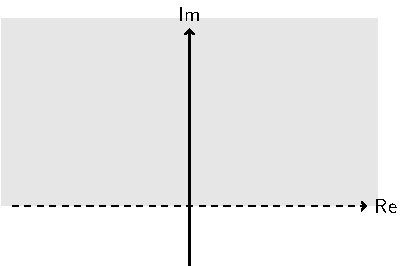
\includegraphics[scale=1]{upperhalf}
%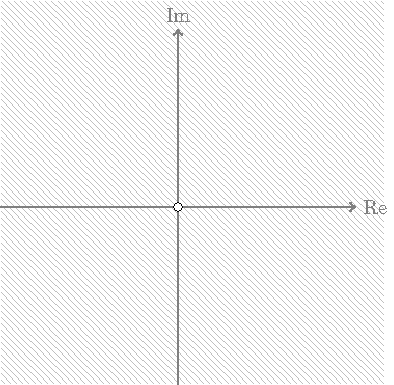
\includegraphics[scale=1]{hplus}
%\vspace*{1cm}
%\includegraphics[scale=1]{sc1}
%\hspace{1cm}
%\includegraphics[scale=1]{sc2}
%\end{center}
%\vspace*{2cm}
%\end{student}
In the proof of Cauchy's Theorem we will need the following fact about the integral of a continuous function $f$ along a smooth path $\Gamma$: if $\tilde{\Gamma}$ denotes the reverse of $\Gamma$ then
\[
\int_{\tilde{\Gamma}} f = - \int_{\Gamma} f.
\]
We shall also fix the following notation: $T(z_1,z_2,z_3)$ denotes the triangle with vertices $z_1,z_2,z_3$, and hence with edges given by the line segments $[z_1,z_2],[z_2,z_3],[z_3,z_1]$.  The boundary of $T$ is denoted by $\partial T$, which defines a closed contour
\[
\partial T = [z_1,z_2] + [z_2,z_3] + [z_3,z_1].
\]
\begin{theorem}[Cauchy's Theorem for a Triangle]
\label{t:cauchyt} Let $f$ be a function that is holomorphic on a simply connected region $\mathcal{R}$ and let $T(z_1,z_2,z_3)$ be a triangle in $\mathcal{R}$ with boundary $\partial T$.  Then
\[
\int_{\partial T} f = 0.
\]
\end{theorem}
\begin{center}
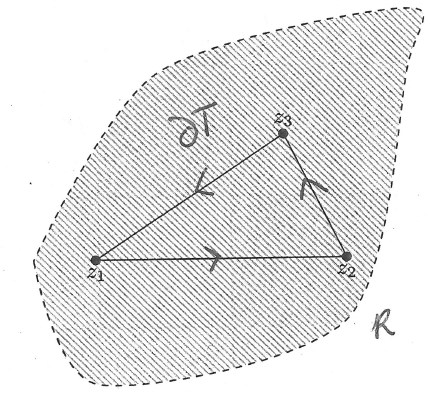
\includegraphics[scale=0.4]{ch4_cauchyt_full}
\end{center}
Note that if we knew that $f$ were to have an antiderivative $F$ on $\mathcal{R}$, then Theorem~\ref{t:closed} would show that
\[
\int_{\partial T} f =0.
\]
Later we will see that in fact $f$ does have an antiderivative on $\mathcal{R}$, but the proof will rely Cauchy's Theorem for a triangle - thus we need to prove Theorem~\ref{t:cauchyt} without this assumption.

Before proving Theorem~\ref{t:cauchyt}, we need the following lemma:
\begin{lemma}
\label{l:cauchyt}
Let $f$ be a function that is holomorphic on a simply connected region $\mathcal{R}$ and let $T(z_1,z_2,z_3)$ be a triangle in $\mathcal{R}$.  Then there exists a nested sequence of triangles $T \supseteq T_1 \supseteq T_2 \supseteq \ldots \supseteq T_n \supseteq \ldots$ with the property that
\[
\frac{1}{4^n} \abs{ \int_{\partial T} f } \leq \abs{ \int_{\partial T_n} f } \text{ and } \ell ( \partial T_n) = \frac{1}{2^n} \ell ( \partial T)
\]
for all $n$. Moreover, there exists a point $z_0 \in \mathcal{R}$ with $z_0 \in T_n$ for all $n$.
\end{lemma}
{\bf Proof }
 Using the midpoints of the sides of $T$, construct four similar triangles $T^{(1)},T^{(2)},T^{(3)}$ and $T^{(4)}$ as shown.

\begin{blankbox}
%\vspace*{2cm}
\begin{center}
\altgraphics[scale=0.6]{ch4_cauchyt2_full}{ch4_cauchyt2}
\end{center}
%\vspace*{2cm}
Then for $j=1,2,3,4$ we have $\ell(\partial T^{(j)}) = \frac{1}{2} \ell ( \partial T)$ by construction.



Note that with all contours taken anticlockwise,
\[
\int_{\partial T^{(1)}} f + \int_{\partial T^{(2)} } f + \int_{\partial T^{(3)}} f + \int_{\partial T^{(4)}} f = \int_{\partial T} f,
\]

as the integrals along the `interior' edges of the $T^{(j)}$ cancel in pairs (this uses $\int_{\tilde{\Gamma}} f = - \int_{\Gamma} f$, where $\tilde{\Gamma}$ is the reverse of $\Gamma$ ):
\begin{center}
\altgraphics[scale=0.6]{ch4_cauchyt3_full}{ch4_cauchyt3}
\end{center}
\end{blankbox}
Moreover, by the triangle inequality
\[
\abs{\int_{\partial T} f} \leq \abs{ \int_{\partial T^{(1)}} f} + \abs{\int_{\partial T^{(2)} } f }+ \abs{\int_{\partial T^{(3)}} f }+ \abs{\int_{\partial T^{(4)}} f }. 
\]
%\vspace*{5cm}
\begin{blankbox}
At least one of these four integrals has modulus greater than or equal to the other three; call the corresponding triangle $T_1$.  Then
\[
\abs{\int_{\partial T} f} \leq \abs{ \int_{\partial T^{(1)}} f} + \abs{\int_{\partial T^{(2)} } f }+ \abs{\int_{\partial T^{(3)}} f }+ \abs{\int_{\partial T^{(4)}} f } \leq 4 \abs{ \int_{\partial T_1} f},
\]
and so
\[
\frac{1}{4} \abs{ \int_{\partial T } f } \leq \abs{\int_{\partial T_1} f}.
\]
\end{blankbox}
Now, use the midpoints of the edges of $T_1$ to get four more triangles, one of which is a triangle $T_2$ satisfying
\[
\frac{1}{4} \abs{ \int_{\partial T_1} f } \leq \abs{ \int_{\partial T_2} f } \quad\text{and}\quad \ell ( \partial T_2) = \frac{1}{2} \ell ( \partial T_1) = \frac{1}{2^2} \ell(\partial T),
\]

\begin{center}
\altgraphics[scale=0.6]{ch4_cauchyt4_full}{ch4_cauchyt4}
\end{center}

\begin{blankbox}
Thus 
\[
\frac{1}{4^2} \abs{ \int_{\partial T} f } \leq \abs{ \int_{\partial T_2} f }.
\]


Continuing in this way we get $T\supseteq T_1 \supseteq T_2 \supseteq \ldots \supseteq T_n \supseteq \ldots$ with 
\[
\frac{1}{4^n} \abs{ \int_{\partial T} f} \leq \abs{ \int_{\partial T_n} f }\quad\text{and}\quad \ell(\partial T_n) = \frac{1}{2^n} \ell ( \partial T)
\]
for each $n$.
\end{blankbox}
\begin{center}
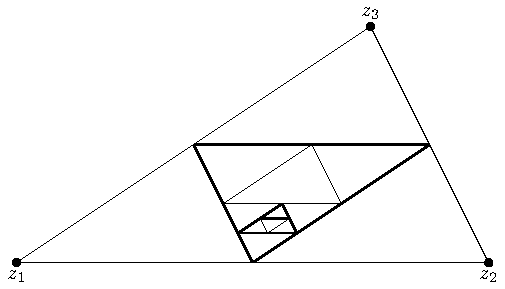
\includegraphics[scale=0.6]{ch4_cauchyt5}
\end{center}


As the sequence is nested, there exists a point $z_0$ with $z_0 \in T_n$ for all $n$, and since $\mathcal{R}$ is simply connected, $z_0 \in \mathcal{R}$.
\qed

We are now in a position to prove Cauchy's Theorem for a Triangle.
\begin{exercise}
Try to prove Cauchy's Theorem for a Triangle, using the following steps.
\begin{enumerate}
\item[(i)] Let $\epsilon >0$ be given.  Use the fact that $f$ is differentiable at $z_0$ to show that there exists $\delta >0$ such that 
\[ 
z \in \mathcal{R},\  \abs{z-z_0} < \delta \Rightarrow \abs{f(z)-f(z_0)-(z-z_0)f'(z_0)} \leq \epsilon \abs{z-z_0}.
\]
\item[(ii)] With $\epsilon$ and $\delta$ as chosen in the previous step, show that there exists $n \in \mathbb{N}$ such that
\[
z \in \partial T_n \Rightarrow \abs{f(z)-f(z_0)-(z-z_0)f'(z_0)} < \epsilon \ell( \partial T_n).
\]
As a hint, first explain why we can choose $n$ with $\ell ( \partial T_n) < \delta$.
\item[(iii)] Show that for any constants $\alpha,\beta \in \C$ we have
\[
\int_{\partial T_n} (\alpha + \beta (z-z_0) )\ dz = 0,
\]
and deduce that
\[
\int_{\partial T_n} f = \int_{\partial T_n} (f(z)-f(z_0)-f'(z_0)(z-z_0))\ dz.
\]
\item[(iv)] Use step (iii) and the Estimation Lemma to show that
\[
\abs{\int_{\partial T_n} f } \leq \epsilon \cdot \frac{1}{4^n} \cdot \brac{\ell(\partial T) }^2.
\]
\item[(v)] Complete the proof.
\end{enumerate}
\end{exercise}
\begin{proof}[of Cauchy's Theorem for a Triangle (Theorem~\ref{t:cauchyt})]
We are going to show that given any $\epsilon>0$ we have
\[
\abs{ \int_{\partial T} f } \leq \epsilon [\ell (\partial T)]^2
\]
where $\ell ( \partial T )$ is the length of the boundary of the triangle $T$.

Let $\set{ T_n}$ be the nested sequence of triangles constructed in Lemma~\ref{l:cauchyt} and $z_0 \in \mathcal{R}$ such that $z_0 \in T_n$ for all $n$.

\emph{Step 1:}    Let $\epsilon>0$ be given.  We will show that there exists $\delta>0$ such that 
\[
\abs{z-z_0}<\delta \Longrightarrow \abs{f(z)-f(z_0)-(z-z_0)f'(z_0)} \leq \epsilon \abs{z-z_0}.
\]


  Since $f$ is holomorphic on $\mathcal{R}$ it is differentiable at $z_0$ with derivative $f'(z_0)$, or in other words
  \[
  \lim_{h \to 0} \frac{f(z_0+h)-f(z_0)}{h} = f'(z_0).
  \]  

  This means that there is some $\delta>0$ such that
  \begin{align*}
  0 < \abs{h} < \delta &\Longrightarrow \abs{ \frac{f(z_0+h)-f(z_0)}{h} - f'(z_0) } < \epsilon \\
  \shortintertext{ or in other words, writing $z=z_0+h$,}
  0 < \abs{z-z_0} < \delta &\Longrightarrow \abs{ \frac{f(z)-f(z_0)}{z-z_0} - f'(z_0) } < \epsilon \\
  & \Longrightarrow \abs{ \frac{f(z)-f(z_0)-(z-z_0)f'(z_0)}{z-z_0} } < \epsilon.
  \end{align*}
Thus
\[
0 < \abs{z-z_0} < \delta \Longrightarrow \abs{f(z)-f(z_0)-(z-z_0)f'(z_0)} < \epsilon \abs{z-z_0}.
\]
If we allow $z=z_0$, this becomes
\[
\abs{z-z_0} < \delta \Longrightarrow \abs{f(z)-f(z_0)-(z-z_0)f'(z_0)} \leq \epsilon \abs{z-z_0}
\]
(since when $z=z_0$, both sides are zero).

\emph{Step 2: } With $\epsilon>0$ as before, and $\delta>0$ as chosen in the previous step, we choose $n$ large enough so that $\ell ( \partial T_n ) < \delta$, which can always be done as $\ell ( \partial T_n ) = \frac{1}{2^n} \ell ( \partial T)$ (note that $n$ depends on $\delta$, which in turn depends on $\epsilon$).

We will show that for $z \in \partial T_n$ we have
\[
\abs{f(z)-f(z_0)-(z-z_0)f'(z_0)}<\epsilon \ell ( \partial T_n).
\]



If $z \in \partial T_n$, then the distance from $z$ to $z_0$ can be no more than the length of the longest edge of $T_n$, which is less than $\ell ( \partial T_n)$.
%\vspace*{5cm}
\begin{center}
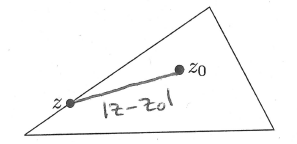
\includegraphics[scale=0.6]{ch4_cauchyt6_full}
\end{center}
%\vspace*{7cm}
Thus
\[
z \in \partial T_n \Longrightarrow \abs{z-z_0} \underbrace{< \ell (\partial T_n) }_{\text{geometry}} \underbrace{< \delta}_{\text{choice of }n},
\]
and hence $T_n \subset D(z_0,\delta)$.

Thus for any $n$ large enough so that $\ell ( \partial T_n) < \delta$, we have
\begin{align*}
z \in \partial T_n \Longrightarrow \abs{f(z)-f(z_0)-(z-z_0)f'(z_0)} &\leq \epsilon \abs{z-z_0} \\
& < \epsilon \ell ( \partial T_n).
\end{align*}
\begin{center}
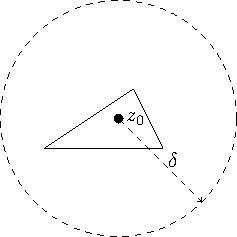
\includegraphics[scale=1]{ch4_cauchyt7}
\end{center}

\emph{Step 3}: We use the Estimation Lemma to find an upper estimate for $\int_{\partial T_n} f$, where $n$ was chosen in the previous step.  

Note that
\[
\int_{\partial T_n} (\alpha+\beta(z-z_0)) dz =0 \text{ for }\alpha,\beta \in \C,
\]
because $z \mapsto \alpha + \beta (z-z_0)$ has an antiderivative $z \mapsto \alpha z + \frac{\beta(z-z_0)^2}{2}$.


This means that
\[
\int_{\partial T_n} {\Big(} \underbrace{f(z_0)}_{\alpha}+\underbrace{f'(z_0)}_{\beta} (z-z_0) {\Big)} dz =0,
\]
and so
\[
\int_{\partial T_n} f = \int_{\partial T_n} {\Big(} f(z)-\underbrace{f(z_0)-f'(z_0)(z-z_0)}_{\text{integral }0\text{ along } \partial T_n} {\Big)} dz
\]
We shall use the Estimation Lemma to find an upper estimate for this integral.  Indeed, we have
\begin{align*}
\abs{\int_{\partial T_n} f} & = \abs{\int_{\partial T_n} \left[ f(z)-f(z_0)-f'(z_0)(z-z_0) \right]\ dz} &&\\
& \leq \epsilon \ell ( \partial T_n ) \ell ( \partial T_n) &&\text{ By step 3} \\
& = \epsilon \left( \frac{1}{2^n} \ell ( \partial T ) \right) \left( \frac{1}{2^n} \ell ( \partial T) \right) && \text{ as } \ell (\partial T_n) = \frac{1}{2^n} \ell ( \partial T) \\
& = \epsilon \frac{1}{4^n} \left[ \ell ( \partial T) \right]^2.
\end{align*}





\emph{Step 4:} Completing the proof.

By Step 3, given any $\epsilon>0$, there is $n$ such that
\[
\abs{ \int_{\partial T_n} f } \leq \epsilon \frac{1}{4^n} \left[ \ell ( \partial T) \right]^2.
\]

In Lemma~\ref{l:cauchyt}, we showed that
\[
\frac{1}{4^n} \abs{ \int_{\partial T} f } \leq \abs{ \int_{\partial T_n} f},
\]
and so combining these facts, we have
\[
\abs{ \int_{\partial T} f } \leq \epsilon \left[ \ell ( \partial T) \right]^2
\]
for all $\epsilon > 0$.  Because $\epsilon>0$ was arbitrary and $\ell ( \partial T)$ is fixed, we get
\[
\abs{ \int_{\partial T} f } = 0, \text{ hence } \int_{\partial T} f =0.
\]

\end{proof}


\begin{example}
Let $f:\C \to \C$ be defined by $f(z)=\sin \left( \exp \left( \cos \left( z^3-4z^2+i \right) \right) \right)$, which is holomorphic on $\C$.  There is no obvious antiderivative for $f$, but nonetheless, Cauchy's Theorem shows us that for any triangle $T$ we have
\[
\int_{\partial T} f = 0.
\]
\end{example}
\begin{example}
Let $f(z) = \dfrac{1}{z}$, which is holomorphic on $\C \backslash \set{0}$.  We shall evaluate $\int_{\partial T} f$ for different triangles $T$: let $T_1$ be a triangle enclosing the origin, and $T_2$ a triangle lying to the left of the imaginary axis as shown.
\begin{center}
\begin{tabular}{cc}
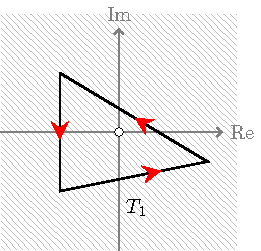
\includegraphics[scale=1]{ch4_cauchytexample1} & 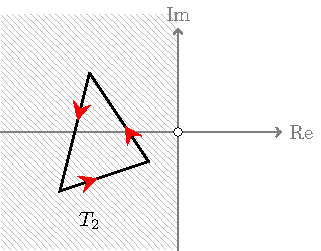
\includegraphics[scale=1]{ch4_cauchytexample2}
\end{tabular}
\end{center}
\end{example}
\begin{solution}
Since $\C \backslash \set{0}$ is not simply connected, Cauchy's Theorem for a triangle tells us nothing about
\[
\int_{\partial T_1} \frac{1}{z}\ dz.
\]
However, $\C \backslash \set{0}$ has simply connected subregions, for example, the left-half plane
\[
\mathcal{L} = \set{ z \in \C : \Re (z) < 0 }.
\]

The triangle $T_2$ is contained in $\mathcal{L}$, so Cauchy's Theorem for a triangle gives
\[
\int_{\partial T_2} \frac{1}{z}\ dz =0.
\]
In fact, if $T$ is any triangle in $\C \backslash \set{0}$ that does not enclose the origin, we can find a simply connected subregion of $\C \backslash \set{0}$ that contains $T$, and conclude that
\[
\int_{\partial T} \frac{1}{z}\ dz =0.
\]
\end{solution}
%\newpage
%\begin{absolutelynopagebreak}
\section{Cauchy's Theorem for Starlit Regions}

\begin{definition}
A region $\mathcal{R}$ is called \emph{starlit} if there is a point $z_{\ast} \in \mathcal{R}$ such that for any $z \in \mathcal{R}$ the line segment $[z_{\ast},z]$ lies inside $\mathcal{R}$.  The point $z_{\ast}$ is called a \emph{star centre} for $\mathcal{R}$.
\end{definition}

The name starlit comes from the idea that the `rays of light' from the `star' $z_{\ast}$ fall on every point of $\mathcal{R}$.  
%\begin{student}
\begin{center}
\altgraphics[scale=1.5]{ch4_starlit1_full}{ch4_starlit1} \\
\blank{The region $\mathcal{R}_1$ on the left is starlit, as any point $z \in \mathcal{R}_1$ can be connected to $z_*$ using the line segment $[z_*,z]$.  The region $\mathcal{R}_2$ on the right is not, since no matter which point we choose as $z_*$, the line segment joining $z_*$ to the point opposite it leaves $\mathcal{R}_2$.}
\end{center}
\begin{tabular}{c m{0.5\textwidth} }
\begin{minipage}{0.5\textwidth}
\centering
\altgraphics[scale=1.5]{ch4_starlit2_full}{ch4_starlit2}
\end{minipage} & \blank{The region $\C \backslash \set{0}$ is not starlit; indeed if $z_*$ were a star centre, then the line segment $[z_*,-z_*]$ would be contained in $\C \backslash \set{0}$, which is not the case for any choice of $z_*$.}
\end{tabular}
\bigskip

\begin{theorem}[The Existence of Antiderivatives on Starlit Regions]
\label{t:starlit}
Let $f$ be holomorphic on a starlit region $\mathcal{R}$ with star centre $z_{\ast} \in \mathcal{R}$.  Then the function $F:\mathcal{R} \to \C$ defined by
\[
F(z) = \int_{[z_{\ast},z]} f
\]
is an antiderivative for $f$ on $\mathcal{R}$.
\end{theorem}

\leftimage{
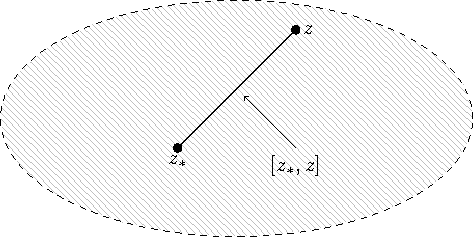
\includegraphics[scale=0.75]{ch4_starlitantid}
}
{
Since $\mathcal{R}$ is starlit, $[z_*,z]$ is contained in $\mathcal{R}$ and so $\int_{[z_*,z]} f$ is well-defined for all $ z \in \mathcal{R}$.
}

\begin{exercise}
Use the following steps to prove this Theorem.
\begin{enumerate}
\item[(i)] Use the definition of $F$, together with Cauchy's Theorem for a Triangle, to show that for $h \in \C$,
\[
F(z_0+h)-F(z_0) = \int_{[z_0,z_0+h]} f.
\]
\item[(ii)] Show that
\[
\frac{F(z_0+h)-F(z_0)}{h} - f(z_0) = \frac{1}{h} \int_{[z_0,z_0+h]} (f(z)-f(z_0)\ dz.
\]
\item[(iii)] Let $\epsilon >0$ be given.  Use the Estimation Lemma to show that there exist $\delta >0$ such that
\[ 
\abs{h} < \delta \Rightarrow \abs{\int_{[z_0,z_0+h]} \brac{f(z)-f(z_0)}\ dz} \leq \epsilon \abs{h}.
\]
(Hint: you will need to use the fact that differentiability implies continuity).
\item[(v)] Combine steps (ii) and (iii) to complete the proof.
\end{enumerate}
\end{exercise}

\begin{proof}
We need to show that for any $z_0 \in \mathcal{R}$, $F'(z_0)$ exists and is equal to $f(z_0)$, or in other words
\[
\lim_{h \to 0} \frac{F(z_0+h)-F(z_0)}{h} = f(z_0).
\]
  Write
\[
\frac{F(z_0+h)-F(z_0)}{h} = \frac{1}{h} \int_{[z_{\ast},z_0+h]} f - \frac{1}{h} \int_{[z_{\ast},z_0]} f.
\]
Since $\mathcal{R}$ is open, for sufficiently small $h$, the triangle $T(z_{\ast},z_0+h,z_0)$ is contained in $\mathcal{R}$.
\begin{center}
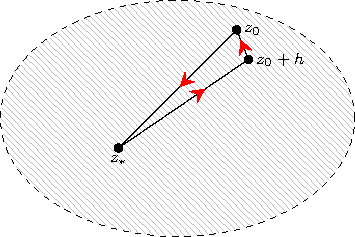
\includegraphics[scale=1]{ch4_starlittriangle}
\end{center}

  Cauchy's Theorem for a Triangle gives
\[
\int_{[z_*,z_0+h]} f + \int_{[z_0+h,z_0]} f + \int_{[z_0,z_*]} f = 0,
\]
hence
\[
\int_{[z_*,z_0+h]}f - \int_{[z_*,z_0]}f = - \int_{[z_0+h,z_0]} f = \int_{[z_0,z_0+h]} f.
\]
This gives
\[
\frac{F(z_0+h)-F(z_0)}{h} = \frac{1}{h} \int_{[z_0,z_0+h]} f.
\]
We now use the fact that
\[
\int_{[z_0,z_0+h]} 1 dz = h,
\]
which implies that
\[
f(z_0) = f(z_0) \cdot \frac{1}{h} \cdot h = f(z_0) \frac{1}{h} \int_{[z_0,z_0+h]} 1 dz = \frac{1}{h} \int_{[z_0,z_0+h]} f(z_0)\ dz
\]
(since $f(z_0)$ is a constant).  Combining this with the previous step, we see that 
%\newpage
%\vspace*{5cm}
%\newpage
\begin{align*}
 \frac{F(z_0+h)-F(z_0)}{h}-f(z_0)  &= \frac{1}{h} \left[ \int_{[z_0,z_0+h]} f(z)\ dz - \int_{[z_0,z_0+h]} f(z_0)\ dz \right] \\
& = \frac{1}{h} \int_{[z_0,z_0+h]} (f(z)-f(z_0))\ dz 
\end{align*}
(since both integrals are along the same path, we can combine them).
%\begin{absolutelynopagebreak}
Hence
\[
\abs{ \frac{F(z_0+h)-F(z_0)}{h}-f(z_0) } = \frac{1}{\abs{h}} \abs{ \int_{[z_0,z_0+h]} (f(z)-f(z_0)) dz }
\]
Now we shall use the Estimation Lemma to obtain an upper estimate for this integral.  It is easy to see that $\ell([z_0,z_0+h]) = \abs{h}$, thus we must find an upper bound for $\abs{f(z)-f(z_0)}$ when $z \in [z_0,z_0+h]$.
%\end{absolutelynopagebreak}


We use the fact that $f$ holomorphic on $\mathcal{R}$ implies $f$ continuous on $\mathcal{R}$, and in particular, continuous at $z_0$.  Hence given any $\epsilon >0$ there is some $\delta >0$ such that
\[
0< \abs{z-z_0} < \delta \Longrightarrow \abs{f(z)-f(z_0)} < \epsilon.
\]
Thus if $\abs{h} < \delta$ then
\begin{align*}
z \in [z_0,z_0+h] & \Longrightarrow \abs{z-z_0} < \abs{h} < \delta \\
& \Longrightarrow \abs{f(z)-f(z_0)} < \epsilon.
\end{align*}
%\newpage
%\vspace*{25cm}
In other words, once $\abs{h}<\delta$, $\epsilon$ is an upper bound for $\abs{f(z)-f(z_0)}$ for $z \in [z_0,z_0+h]$.  Thus the Estimation Lemma gives the upper estimate
\[
\abs{ \int_{[z_0,z_0+h]} \left( f(z)-f(z_0) \right)\ dz } \leq \epsilon \abs{h}
\]
whenever $\abs{h} < \delta$.

Thus given any $\epsilon>0$ there is $\delta>0$ such that
\begin{align*}
0 < \abs{h} < \delta \Longrightarrow 
\abs{ \frac{F(z_0+h)-F(z_0)}{h}-f(z_0) } & = \frac{1}{\abs{h}} \abs{ \int_{[z_0,z_0+h]} (f(z)-f(z_0) dz } \\
& \leq \frac{1}{\abs{h}} \epsilon \abs{h} = \epsilon.
\end{align*}
But this is equivalent to saying
\[
\lim_{h \to 0} \frac{F(z_0+h)-F(z_0)}{h} = f(z_0),
\]
or in other words, $F'(z_0)=f(z_0)$, as required.
%\vspace*{8cm}

\end{proof}
\begin{theorem}[Cauchy's Theorem for Starlit Regions]
\label{t:cauchyst}
Let $f$ be a function that is holomorphic in a starlit region $\mathcal{R}$ and let $\mathcal{C}$ be a closed contour in $\mathcal{R}$.  Then
\[
\int_{\mathcal{C}} f = 0.
\]
\end{theorem}
\begin{blankbox}
{\bf Proof}
By Theorem~\ref{t:starlit}, $f$ has an antiderivative in $\mathcal{R}$.  Thus by Theorem~\ref{t:closed}
\[
\int_{\mathcal{C}} f = 0.
\]
\qed
\end{blankbox}

In fact, Cauchy's Theorem extends to more general regions, as we shall see later.

\section{Application: The Complex Logarithm and Power Functions}

In this section we will define the Complex Logarithm and Power functions.


Consider the Real function $f:(0,+\infty) \to \R$ defined by $f(x) = \dfrac{1}{x}$. Since $f$ is continuous on $(0,+\infty)$, the Fundamental Theorem of Calculus ensures that $f$ has an antiderivative on $(0,+\infty)$.  One way of defining the \emph{natural logarithm} function, is to define it as an antiderivative of $\dfrac{1}{x}$ on $(0,+\infty)$:
\begin{equation}
\label{e:reallog}
\log (x) = \int_1^x \frac{1}{t}\ dt \quad \text{ for all } x \in (0,+\infty).
\end{equation}
\begin{note}
\begin{enumerate}
\item[(i)] There are of course other ways of defining $\log (x)$ for $x \in (0,+\infty)$, most commonly as the inverse of the exponential function $\exp:\mathbb{R} \to (0,+\infty)$.  This definition is equivalent.
\item[(ii)]  The Fundamental Theorem of calculus actually tells us that for \emph{any} choice of $a \in (0,+\infty)$, the function $F: (0,+\infty) \to \mathbb{R}$ defined by
\[
F(x) = \int_a^x \frac{1}{t}\ dt
\]
is an antiderivative for $x \mapsto \frac{1}{x}$.  However, we must take $a=1$ to ensure that $F$ is indeed the inverse of $x \mapsto e^x$: since $e^0=1$ we want $\log (1)=0$.
\end{enumerate}
\end{note}
We shall generalise~\eqref{e:reallog} to define the Complex Logarithm function, using Theorem~\ref{t:starlit} (the existence of antiderivatives on starlit regions).  The function
\[
f(z) = \frac{1}{z}\quad (z \in \C \backslash \set{0})
\]
is holomorphic on $\C \backslash \set{0}$. However, this set is neither simply connected nor starlit.  Therefore, we will restrict our attention to the subset
\[
\C_{\pi} = \set{ z \in \C: z \neq 0 \text{ and } \Arg(z) \neq \pi },
\]
which is both starlit and simply connected. 
\begin{center}
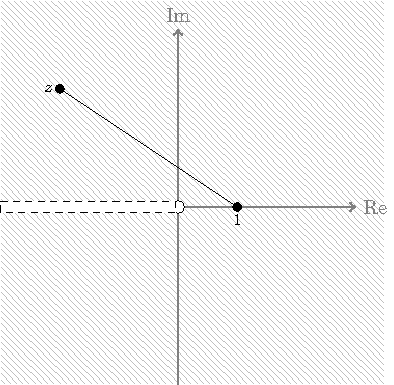
\includegraphics[scale=1]{ch4_cpi2}
\end{center}
 The point $1$ on the real axis is a star centre for $\C_{\pi}$ - in particular, this allows us to apply Theorem~\ref{t:starlit} to conclude that
\[
z \mapsto \int_{[1,z]} \frac{1}{\zeta}\ d \zeta
\]
is an antiderivative for $z \mapsto \frac{1}{z}$ on $\C_{\pi}$.  We use the variable $\zeta$ (zeta) as the variable of integration because $z$ has been used already.

\begin{definition}
The \emph{Complex Logarithm} function $\Log : \C_{\pi} \to \C$ is defined by
\[
\Log (z) = \int_{[1,z]} \frac{1}{\zeta}\ d \zeta\quad \text{ for } z \in \C_{\pi}.
\]
It is holomorphic on $\C_{\pi}$.
\end{definition}
In other words, to find the value of $\Log (z)$ we need to evaluate the integral
\[
\int_{[1,z]} \frac{1}{\zeta}\ d \zeta.
\]
We can do this directly by choosing a parametrisation of the path $[1,z]$, however, it is much easier to obtain an alternative definition using the following example.
\begin{example}
We shall show that for all $z \in \C_{\pi}$ we have
\[
\Log(z) = \log ( \abs{z} ) + i \Arg (z)
\]
where $\log:(0,+\infty) \to \R$ denotes the real (natural) logarithm and $\Arg$ is the principal value of the argument.
\end{example}
\begin{solution}
Since the function $f$ defined by $f(z)=\frac{1}{z}$ has an antiderivative on $\C_{\pi}$, the Contour Independence Theorem (Theorem~\ref{t:contint}) tells us that
$\displaystyle \int_{\mathcal{C}} f = \int_{[1,z]} f$ for any contour $\mathcal{C}$ in $\C_{\pi}$ that starts at $1$ and ends at $z$.
\begin{center}
\altgraphics[scale=1]{ch4_logpath}{ch4_cpi2}
%{logpath_full}{cpi3}
\end{center}
We shall use the contour $\mathcal{C}=\Gamma_1+\Gamma_2$, where $\Gamma_1=[1,\abs{z}]$ is the straight line segment along the real axis from $1$ to $\abs{z}$, and $\Gamma_2$ is the arc of the circle with centre $0$ and radius $\abs{z}$ from the point $\abs{z}$ on the positive real axis to $z$. 

Parametrise $\Gamma_1$ with $\gamma_1:[1,\abs{z}] \to \C$, $\gamma_1(t)=t$, and $\Gamma_2$ with $\gamma_2:[0,\Arg (z)] \to \C,$
\[
\gamma_2(t) = \polar{\abs{z}}{t}
\]
Note that $\Gamma_2$ is a path from $\gamma_2 (0) = \abs{z}$ to $\gamma_2 ( \Arg (z)) = z$, hence is traversed 
\begin{itemize}
\item anticlockwise if $\Arg (z) \geq 0$, and
\item clockwise if $\Arg(z)<0$,
\end{itemize}
which ensures that we stay within $\C_{\pi}$.  

We have $\gamma_1'(t)=1$ and $\gamma_2'(t) =  i \gamma_2 (t)$, and so
\begin{align*}
\Log (z) & = \int_{\Gamma_1} \frac{1}{\zeta}\ d\zeta + \int_{\Gamma_2} \frac{1}{\zeta}\ d\zeta \\
& = 
\int_{1}^{\abs{z}} \frac{1}{t}\ dt + \int_0^{\Arg (z)} \frac{1}{\gamma_2(t)} \gamma_2'(t)\ dt \\
& = \left[ \log \abs{t} \right]_1^{\abs{z}} + \int_0^{\Arg (z)} i\ dt \\
& = \log \abs{z} + i \Arg (z).
\end{align*}
\end{solution}
%\vspace*{20cm}
This yields the following alternative definition of the Complex Logarithm function:
\begin{equation}
\Log (z) = \log ( \abs{z} )+i \Arg (z) \quad (z \in \C_{\pi}).
\end{equation}
\begin{note}
This definition of $\Log (z)$ uses the principal value of the argument - that is to say, our definition depends on us taking $\arg (z) \in (-\pi, \pi]$.  For this reason it is sometimes called the \emph{principal branch} of the (complex) Logarithm function.  Other `branches' (i.e. other definitions) of $\Log (z)$ are possible by taking different values of the argument.
\end{note}
\begin{example}
Compute the following principal logarithms: $\Log (7)$, $\Log (-2i)$ and $\Log (1+i)$.
\end{example}
\begin{solution}
\begin{align*}
\Log (7) & = \log \abs{7} + i \Arg (7) = \log(7) \\
\Log (-2i) & = \log \abs{-2i} + i \Arg (-2i) \\
& = \log(2) -i \frac{\pi}{2} \\
\Log (1+i ) & = \log \abs{1+i} + i \Arg (1+i) \\
& = \log ( \sqrt{2} ) + i \frac{\pi}{4} \\
& = \frac{1}{2} \log (2) + i \frac{\pi}{4.}
\end{align*}
\end{solution}

So far, $\Log (z)$ is defined (and is holomorphic) on $\C_{\pi}$. We can extend the domain of $\Log$ to $\C \backslash\set{0}$ by defining it on the negative real axis, where points have principal argument $\pi$, as follows:
\[
\Log (z) = \log \left( \abs{z} \right) + i \pi, \mbox{ for $z \neq 0$ on the negative real axis.}
\]
\begin{question}
Is $\Log(z)$ continuous on $\C \backslash \set{0}$?
\end{question}
\begin{answer}
%\begin{center}
%\altgraphics[scale=0.4]{log_discontinuous_full}{cless0}
%\end{center}
For $t$ on the negative real axis,
\[
\rlim{z \to t}{ \Im (z) > 0 } \Arg (z) = \pi, \text{ while} \rlim{z \to t}{\Im(z)<0} \Arg (z) = -\pi.
\]
Thus $z \mapsto \Arg (z)$ is discontinuous on the negative real axis.  Since $\Arg (z)$ is the imaginary part of $\Log(z)$, it follows that $\Log$ is also discontinuous on the negative real axis.
\end{answer}


\begin{question}
Is $\Log$ the inverse of $\exp$?
\end{question}
\begin{answer}
Not exactly.  For any $z \in \C \backslash \set{0}$, we have
\begin{align*}
\exp ( \Log (z)) & = \exp \left( \log ( \abs{z} ) + i \Arg (z) \right) \\
& = e^{\log \abs{z}} \left( \cos ( \Arg (z))+i \sin ( \Arg (z) ) \right) \\
& = \underbrace{\abs{z}\left( \cos ( \Arg (z))+i \sin ( \Arg (z) ) \right)}_{\text{Polar form of }z} \\
& = z.
\end{align*}
However, $\exp:\C \to \C$ is not injective (e.g. $\exp(0)=\exp(i2\pi)=1$), thus we cannot have $\Log ( \exp(z)) = z$ for all $z$.  We do have
\begin{align*}
\Log ( \exp (x+iy ) ) & = \log \abs{\exp(x+iy)} + i \Arg (\exp(x+iy)) &&\\
& = \log(e^x) + i (y-2k\pi) && \text{ for some }k \in \mathbb{Z} \\
\end{align*}
Hence $\Log (\exp(z))=z$ if and only if $-\pi<\Im(z) \leq \pi$.
%\newpage
%\vspace*{10cm}
\end{answer}



We have seen already how to take roots of complex numbers. We will now extend this definition to \emph{complex} powers of complex numbers, allowing us to compute expressions such as
\[
2^{i}, i^{i}, (1+3i)^{1-i}
\]
and so on. 
\begin{blankbox}
 The following observation about powers of real numbers may be useful: suppose we want to find the value of $x^a$ for some $a,x \in \mathbb{R}$ with $x>0$.  We know that
\[
\log (x^a) = a \log (x),
\]
and since $e^{\log(y)}=y$ for all $y \in (0,+\infty)$, we have
\[
x^a = e^{  \log \left( x^a \right) } = e^{  a \log (x) }.
\]
Thus we may take $e^{ a \log (x) }$ to be the definition of $x^a$.
\end{blankbox}
\begin{definition}
\label{d:ppower}
For $\alpha \in \C$, the \emph{Principal $\alpha^{th}$ Power Function} is defined by
\[
z^{\alpha} = \exp \left( \alpha \Log (z) \right)
\]
for all $z \in \C \backslash \set{0}$.
\end{definition}
Because $\Log$ is holomorphic on $\C_{\pi}$ and $\exp$ is holomorphic on $\C$, the Principal Power function is holomorphic on $\C_{\pi}$.  `Principal' refers to the fact that we have used the principal branch of the Logarithm function to define the power function - taking different branches of the Logarithm function will give different power functions.

\begin{example}
 Let us verify that $i^2=-1$ agrees with Definition~\ref{d:ppower}.
\end{example}
\begin{solution}
Indeed, we have
\begin{align*}
i^2 = \exp \left( 2 \Log (i) \right) & = \exp \left( 2 \left[ \log \abs{i}+i \Arg(i) \right] \right) \\
& = \exp \left( 2 \left[ \log(1)+i \frac{\pi}{2} \right] \right) \\
& = \exp(i\pi) = -1.
\end{align*}
\end{solution}
%\vspace*{7cm}



\begin{example}
Calculate $2^i$ and $(1+i)^{-i}$.
\end{example}
\begin{solution}
This time, we have
\begin{align*}
2^i = \exp(i \Log(2) ) & = \exp(i \log (2) ) \\
& = \cos(\log(2))+i \sin(\log(2))
\end{align*}
and
\begin{align*}
(1+i)^{-i} & = \exp \left( -i \Log (1+i) \right) \\
& = \exp \brac{-i\brac{\tfrac{1}{2}\log(2)+i\frac{\pi}{2}}} \\
& = \exp \brac{\tfrac{\pi}{4}-i\tfrac{1}{2}\log(2)} \\
& = \polar{e^{\pi/4}}{\tfrac{1}{2}\log(2)}.
\end{align*}
\end{solution}




